\documentclass[
  aspectratio=169,
  xcolor={svgnames},
  hyperref={colorlinks,citecolor=DarkBlue,urlcolor=DarkBlue,linkcolor=DarkBlue},
  hideallsubsections
]{beamer}
\usepackage[T2A]{fontenc}
\usepackage[russian]{babel}
\usepackage{float}
\usepackage{mathtools}
\usepackage{smartref}
\usepackage{gensymb}
\usepackage{textcomp}
\usepackage{tabularray}
\usepackage{csquotes}
\usepackage{fixmath}
\usepackage{amsmath}
\usepackage{arcs}
\usepackage{wasysym}
\everymath{\displaystyle}

\let\Im\relax
\let\Re\relax
\DeclareMathOperator{\Re}{Re}
\DeclareMathOperator{\Im}{Im}

\DeclareMathOperator{\grad}{grad}
\DeclareMathOperator{\rot}{rot}
\DeclareMathOperator{\Div}{div}

\renewcommand{\vec}[1]{\mathbold{#1}}

\newcommand{\Real}{\mathbb{R}}
\newcommand{\Complex}{\mathbb{C}}

\usepackage{biblatex}
\addbibresource{src/bibliography.bib}

\setbeamertemplate{caption}[numbered]
\setbeamertemplate{navigation symbols}{}

\usepackage{tikz}


\title[РГР по матанализу]
{Расчетно-графическая работа по математическому анализу}
\subtitle{Вариант 5}
\author[Гайдеров, Терехин, Цалов, Щетинин]
{Гайдеров Ярослав \and Терехин Никита \and Цалов Василий \\ \and Щетинин Станислав}
\institute[ИТМО]{Университет ИТМО}
\date[2023 г.]{Декабрь 2023}
\usetheme{Goettingen}


\begin{document}
\frame{\titlepage}

\section{Задание 1. Потенциал векторного поля}
\begin{frame}\frametitle{Задание 1. Потенциал векторного поля}
	Дано векторное поле \( \vec H = \left( 1; \frac{-1}{y^2} \right) \).

	План:
	\begin{enumerate}
		\item Убедитесь, что поле потенциально
		\item Найдите уравнения векторных линий
		\item Изобразите векторные линии на рисунке
		\item Найдите потенциал поля при помощи криволинейного интеграла
		\item Изобразите линии уровня потенциала (эквипотенциальные линии).
		      Проиллюстрируйте ортогональность линий уровня и векторных линий.
		\item Зафиксируйте точки \( A \) и \( B \) на какой-либо векторной линии.
		      Вычислите работу поля вдоль этой линии.
	\end{enumerate}
\end{frame}

\subsection{Потенциальность поля}
\begin{frame}\frametitle{Потенциальность поля}
	\begin{block}{Условие потенциальности поля:}
		\[rot \(\vec H\) = 0\]
		\[
			rot \vec H = \left( \frac{\partial H_x}{\partial y} - \frac{\partial H_y}{\partial x} \right) \(\vec k\)
		\]
		\[
			\frac{\partial H_x}{\partial y} = \frac{\partial H_y}{\partial x}
		\]
		\[
			\frac{\partial H_x}{\partial y} = \frac{\partial (1)}{\partial y} = 0
			\qquad
			\frac{\partial H_y}{\partial x} = \frac{\partial ( -\frac{1}{y^2} )}{\partial x} = 0
		\]
	\end{block}
	
	Следовательно, поле потенциально на \(\Real^2\).

\end{frame}

\subsection{Уравнение векторных линий}
\begin{frame}\frametitle{Уравнения векторных линий}
	Решим следующее дифф уравнение:
	\begin{equation*}
		Q(x, y)dx = P(x, y)dy
		\label{eq:vec_lines_definition}
	\end{equation*}
	\begin{equation*}
		-\frac{1}{y^2}dx = dy
		\label{eq:vec_lines_podst}
	\end{equation*}
	Возьмем интеграл от левой и правой частей:
	\begin{equation*}
		-\int \frac{1}{y^2} \, dx = \int \, dy
		\label{eq:vec_lines_int}
	\end{equation*}
	Искомое уравнение имеет вид:
	\begin{align*}
		y + \frac{1}{y^2}x = C
		\label{eq:vec_lines_integrated}
	\end{align*}

\end{frame}

\subsection{Рисунок векторных линий}
\begin{frame}\frametitle{Векторные линии}

	\begin{figure}
		\centering
		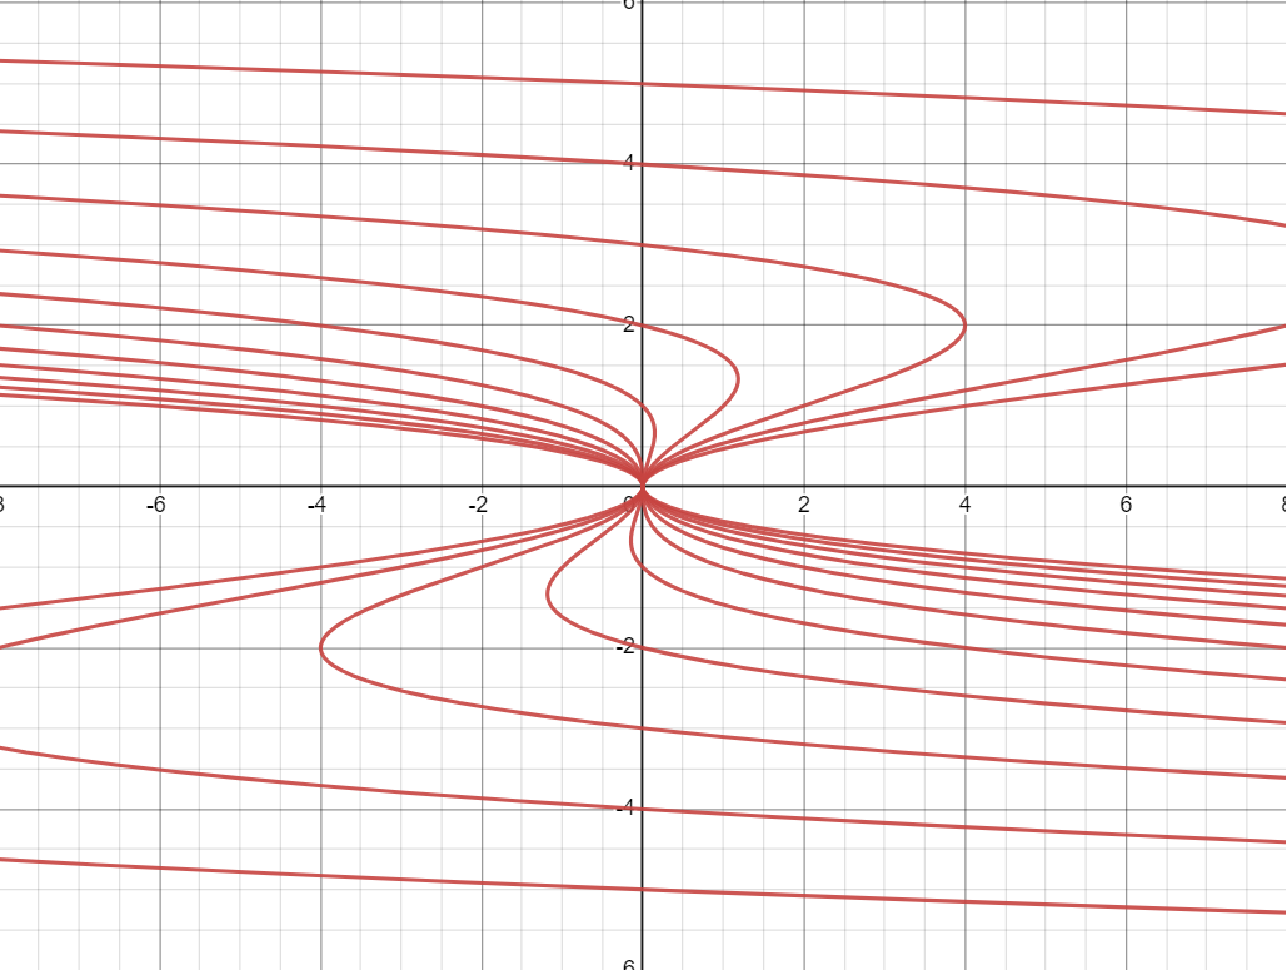
\includegraphics[width=0.5\textwidth]{figures/vec_lines_plot.pdf}
		\caption{Векторные линии поля \(\vec H\)}\label{fig:vec_lines}
	\end{figure}

\end{frame}

\subsection{Потенциал векторного поля}
\begin{frame}\frametitle{Потенциал векторного поля}
	\(U\) -- потенциал поля \(\vec H\). \\
	Возьмем одну точку с фиксированными координтатами
	$(x_0, y_0)$, а другую с переменными - $(x, y)$. \\
	Найдем потенциал по формуле:
	\begin{equation}
		U =
		\int\limits_{x_0}^{x} H_xdx + \int\limits_{y_0}^{y} H_ydy
		\label{eq:u_integral}
	\end{equation}

	\begin{align*}
		U =
		\int\limits_{x_0}^{x} 1dx -
		\int\limits_{y_0}^{y} \frac{1}{y^2} dy = 
		x - x_0 + C_1 - (-\frac{1}{y} + \frac{1}{y_0} + C_2) =
		x + \frac{1}{y} + C
	\end{align*}
	

\end{frame}
\subsection{Линии уровня потенциала}
\begin{frame}\frametitle{Линии уровня потенциала}
	Зелеными линиями изображен $x + \frac{1}{y} = C$
	\begin{figure}
		\centering
		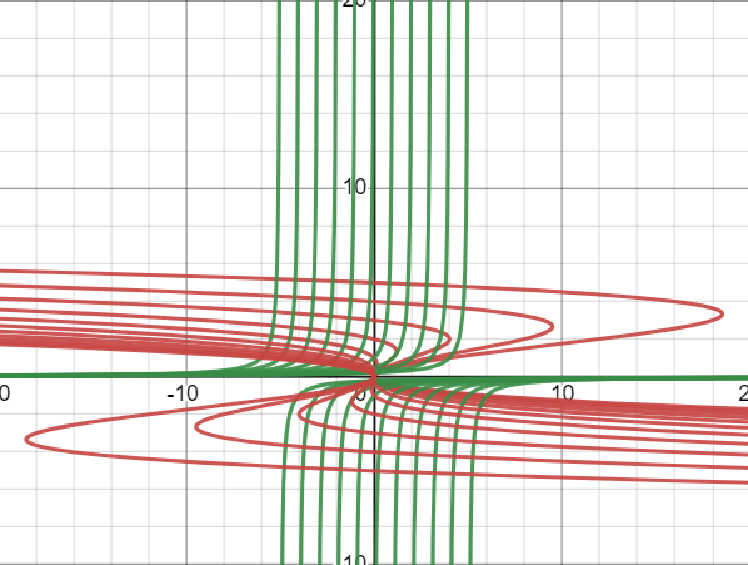
\includegraphics[width=0.5\textwidth]{figures/potential_lines_plot.pdf}
		\caption{Линии уровня потенциала поля \(\vec H\)}\label{fig:potential_lines}
	\end{figure}

\end{frame}

\subsection{Работа поля вдоль линии}
\begin{frame}\frametitle{Работа поля вдоль линии}
	За точку $A$ возьмем $(0, 1)$ за $B - (0.125, 0.5)$
	Работа поля $H$ вдоль векторной линии через это поле равна: 
	\begin{align*}
		\int\limits_{AB} \vec H \, d \vec s
		 & =
		U(B) - U(A)
		=
		(B_x + \frac{1}{B_y}) - (A_x + \frac{1}{A_y}) = \\
		 & = (0.125 + \frac{1}{0.5}) - (0 + \frac{1}{1}) = 1.125
		\label{eq:work_across_line}
	\end{align*}
	\begin{figure}
		\centering
		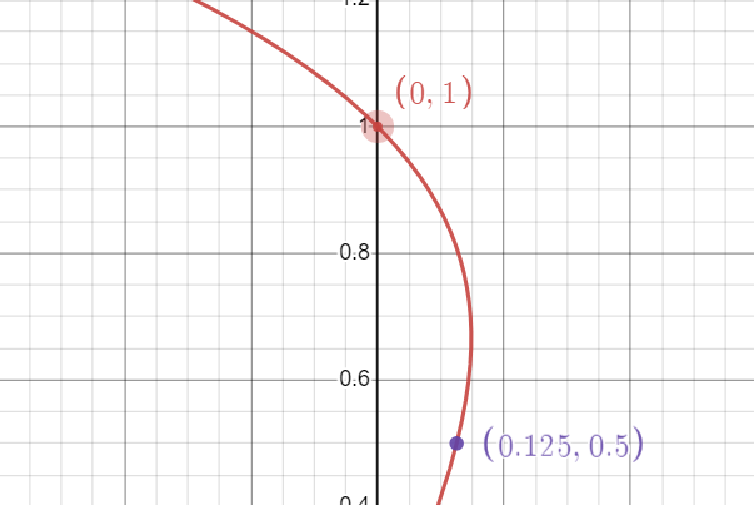
\includegraphics[width=0.5\textwidth]{figures/potential_work.pdf}
		\caption{Работа вдоль линии}\label{fig:potential_work}
	\end{figure}
\end{frame}



\section{Задание 2. Поток векторного поля}
%Task 
\begin{frame}
	\frametitle{Задание 2. Поток векторного поля}

	Дано тело \(T\), ограниченное следующими поверхностями:

	\begin{equation*}
		y + \sqrt{x^2 + z^2} = 0 \qquad x^2+z^2 = 1 \qquad x^2 + y + z^2 = 2
	\end{equation*}

	\begin{figure}
		\centering
		\includegraphics[width=0.6\textwidth]{figures/2_vec_field_body.pdf}
		\caption{Сечение тела \( T \) координатной плоскостью \(Oyz\) }\label{fig:task2_img}
	\end{figure}
\end{frame}

\begin{frame}
	\frametitle{Задание 2. Поток векторного поля}

	Дано тело \(T\), ограниченное следующими поверхностями:

	\begin{equation*}
		y + \sqrt{x^2 + z^2} = 0 \qquad x^2+z^2 = 1 \qquad x^2 + y + z^2 = 2
	\end{equation*}

	\begin{itemize}
		\item Изобразите тело \(T\) на графике в пространстве.
		\item Вычислите поток поля
		      \begin{equation*}
			      \vec a = (\sin zy^2) \vec i + \sqrt{2} x \vec j + (\sqrt{2+y} -3z) \vec k
		      \end{equation*}
		      через боковую поверхность тела \(T\), образованную вращением дуги \(AFEDC\)
		      вокруг оси \(Oy\), в направлении внешней нормали поверхности тела \(T\).
	\end{itemize}

\end{frame}

\subsection{Тело T на графике в пространстве}
\begin{frame}\frametitle{Тело \(T\) на графике в пространстве }

	\begin{figure}
		\centering
		\includegraphics[width=0.65\textwidth]{figures/2_vec_field_3d_img.pdf}
		\caption{Тело \(\vec T\) в пространстве}\label{fig:vec_field_graph}
	\end{figure}

\end{frame}

\begin{frame}\frametitle{Элементы тела \(T\) на графике в пространстве}

	\begin{figure}[ht]
		\centering
		\begin{minipage}{.48\textwidth}
			\centering
			\includegraphics[width=\linewidth]{figures/2_bottom.pdf}
			\caption{Замкнутое дно тела \(\vec T\) в пространстве}
			\label{fig:vec_field_bottom}
		\end{minipage}\hfill
		\begin{minipage}{.48\textwidth}
			\centering
			\includegraphics[width=\linewidth]{figures/2_rotated_surface.pdf}
			\caption{Поверхность вращения дуги AFEDC вокруг оси \(Oy\)}
			\label{fig:vec_field_rotated_surface}
		\end{minipage}
	\end{figure}

\end{frame}



\subsection{Вычисление потока поля}
\begin{frame}\frametitle{Вычисление потока поля}
	Для нахождения искомого потока, найдем поток через тело вращения
	(Рис. \ref{fig:vec_field_rotated_surface}) и вычтем из него поток
	через конусовидное дно, которое замкнем плоскостью \(y = -1\) (Рис. \ref{fig:vec_field_bottom}):

	\begin{equation*}
		\Phi = \Phi_{\text{вращения}} - \Phi_{\text{дна}}
	\end{equation*}

	Так как в обеих случаях тела замкнуты, то для нахождения
	потока поля через них воспользуемся теоремой \textit{Остроградского -- Гаусса}:
	\begin{equation*}
		\oiint\limits_{\Sigma}\left( \vec {a}, \vec {n} \right) \, d\sigma = \iiint\limits_V \Div \vec {a} \, dx \, dy \, dz
	\end{equation*}

	Найдем дивергенцию:
	\begin{equation*}
		\Div \vec a = \frac{\partial a_x}{\partial x} +  \frac{\partial a_y}{\partial y} +  \frac{\partial a_z}{\partial z} = 0 + 0 - 3 = -3
	\end{equation*}
\end{frame}

\begin{frame}\frametitle{Вычисление потока поля: тело вращения}
	Вычислим поток через тело вращения.
	Перейдем к цилиндрическим координатам:
	\begin{equation*}
		\begin{cases}
			x = r \cdot \cos \theta \\
			y = y                   \\
			z = r \cdot \sin \theta
		\end{cases}
	\end{equation*}

	Расставим пределы интегрирования:
	\begin{align*}
		r \in [0, 1], \
		\theta \in [0, 2\pi], \
		y = 2 - x^2 - z^2 = 2 - r^2
	\end{align*}

	Тогда
	\begin{align*}
		\Phi_{\text{вращения}} & = \oiint\limits_{\Sigma}\left( \vec {a}, \vec {n} \right) d\sigma = \iiint\limits_V -3 dV
		= -3 \int\limits_{0}^{2 \pi} d \theta
		\int\limits_{0}^{1} r~dr
		\int\limits_{0}^{2-r^2} dy =                                                                                       \\
		                       & = -3 \int\limits_{0}^{2 \pi} d \theta
		\int\limits_{0}^{1} (2-r^2)r~dr
		= -3 \cdot 2 \pi \cdot
		\left(1 - \frac{1}{4}\right)
		= - \frac{9}{2}\pi
	\end{align*}
\end{frame}

\begin{frame}\frametitle{Вычисление потока поля: дно тела}

	Расставим пределы интегрирования для конусовидного дна тела:
	\begin{align*}
		r \in [0,1] \
		\theta \in [0, 2\pi] \
		y = -\sqrt{x^2 + z^2} = -\sqrt{r}
	\end{align*}

	Тогда
	\begin{align*}
		\Phi_{\text{дна}}
		 & =  \oiint\limits_{D}\left( \vec {a}, \vec {n} \right) d\sigma = \iiint\limits_D -3 dD
		= -3 \int\limits_{0}^{2 \pi} d \theta
		\int\limits_{0}^{1} r~dr
		\int\limits_{-\sqrt{r}}^{0} dy =                                                         \\
		 & = -3 \int\limits_{0}^{2 \pi} d \theta
		\int\limits_{0}^{1}r^{\frac{3}{2}}~dr
		= -3 \cdot 2 \pi \cdot \frac{2}{5} = - \frac{12}{5} \pi
	\end{align*}

	\begin{equation*}
		\Phi =
		\Phi_{\text{вращения}} - \Phi_{\text{дна}} =
		-\frac{9}{2}\pi - \left(- \frac{12}{5} \pi\right) = - \frac{21}{10} \pi
	\end{equation*}
\end{frame}


\subsection{Вывод по задаче}
\begin{frame}\frametitle{Вывод по задаче}
	\begin{itemize}
		\item Изобразили тело \(T\) на графике в трехмерном пространстве.

		\item Нашли дивергенцию векторного поля \(\Div \vec a\) = -3.

		\item Вычислили поток векторного поля через боковую поверхность тела \(\Phi = -\frac{21}{10}\pi \)
	\end{itemize}

\end{frame}



\section{Задание 3. Конформные отображения}
\begin{frame}\frametitle{Задание 3. Конформные отображения}
	\begin{equation*}
		w(z) = \frac{z-1}{z+1} = 1 - \frac{2}{z+1}
	\end{equation*}

	План выполнения работы:
	\begin{enumerate}
		\item Рассмотреть конформное отображение.
		      Определить особые точки отображения (при наличии) и указать их вид.

		\item Изобразить на комплексной плоскости отображение
		      области виртуального пространства в область физического пространства
		      с помощью заданного преобразования.

		\item Выделить действительную и мнимую части отображения
		      для построения искривленной координатной сетки в физическом пространстве.

		\item Взять обратное преобразование к заданному и проанализировать его

		\item Рассчитать профиль показателя преломления используя конформное отображение

	\end{enumerate}
\end{frame}

\subsection{Особые точки}
\begin{frame}\frametitle{Особые точки}
	Отображение имеет две особые точки \(z_1 = 1\) и \(z_2 = -1\).
	Определим их вид.
	Для этого найдем производную \(w'(z)\).

	\[
		w'(z) = \frac{2}{(z+1)^2}
		\qquad
		w(z_1) = w(1) = 0
		\quad
		w'(z_1) = w'(1) \neq 0
	\]
	Значит точка \(z_1 = 1\) является простым нулем.
	Определим вид точки \(z_2 = -1\).

	\[ \lim_{z \to -1} \frac{z-1}{z+1} = \infty \]

	Для функции \(g(z) = 1/w(z) = \frac{z+1}{z-1}\)
	точка \(z_2 = -1\) является простым нулем.
	Значит точка \(z_2 = -1\) является для функции \(w(z)\) полюсом первого порядка.

	Таким образом, отображение является конформным за исключением точки \(z = -1\)
\end{frame}

\subsection{Im(z) и Re(z)}
\begin{frame}{\(\Im w(z)\) и \(\Re w(z)\)}
	Для дальнейшего изучения отображения найдем \( \Im(w(z)) \) и \( \Re(w(z)) \).
	Пусть \( z = u + i v \). Тогда:

	\begin{align*}
		w(z) & = w(u + iv) = 1 - \frac{2}{(u + 1) + iv} = 1 - \frac{2((u + 1) - iv)}{((u+1)+iv)((u+1)-iv)} = \\
		     & = 1 - \frac{2(u + 1 - iv)}{(u+1)^2 + v^2} = 1 - \frac{2u + 2 - 2iv}{u^2 + 2u + v^2 + 1} =     \\
		     & = 1 - \frac{2u+2}{u^2+2u+v^2+1} - i\frac{2v}{u^2+2u+v^2+1} =                                  \\
		     & = \frac{u^2 +v^2 - 1}{u^2+2u+v^2+1} - i \frac{2v}{u^2+2u+v^2+1}
	\end{align*}

	Значит \( \Re(w(z)) = \frac{u^2+v^2-1}{u^2+2u+v^2+1} \), \( \Im(w(z)) = - \frac{2v}{u^2+2u+v^2+1} \)
\end{frame}

\subsection{Точка}
\begin{frame}\frametitle{Точка}
	Изучим, как под действием отображения изменяется точка на плоскости.

	По \href{https://www.geogebra.org/calculator/dncbzxhp}{ссылке} можно перейти на
	демонстрацию Geogebra, на которой находится точка \(A\) в виртуальном пространстве
	и соответствующая ей точка \(A' = w(A)\) в физическом пространстве.

	С включенным режимом трассировки, можно перемещать точку \(A\) и
	изучать, во что переходит соответствующая фигура.
\end{frame}



\subsection{Координатная сетка}
\begin{frame}\frametitle{Координатная сетка}
	Изучим, как под действием отображения изменяется координатная сетка:
	\begin{enumerate}
		\item Построим в виртуальном пространстве множество точек
		      \(v = C\)~--~горизонтальные прямые и \(u = C\)~--~вертикальные прямые
		\item Применим к этим точкам преобразование
		\item Изобразим получившиеся точки в физическом пространстве
	\end{enumerate}

	В приведенных на следующих слайдах графиках константа \(C \in \{-2, -1, -0.5, 0, 0.5, 1, 2\}\)
\end{frame}

\begin{frame}{Координатная сетка (горизонтальные прямые)}
	\begin{figure}
		\centering
		\includegraphics[width=0.9\textwidth]{figures/conformal_grid_horizontal.pdf}
		\caption{Координатная сетка (горизонтальные прямые)}\label{fig:conformal_grid_horizontal}
	\end{figure}
\end{frame}

\begin{frame}{Координатная сетка (вертикальные прямые)}
	\begin{figure}
		\centering
		\includegraphics[width=0.9\textwidth]{figures/conformal_grid_vertical.pdf}
		\caption{Координатная сетка (вертикальные прямые)}\label{fig:conformal_grid_vertical}
	\end{figure}
\end{frame}


\begin{frame}{Координатная сетка}
	\begin{figure}
		\centering
		\includegraphics[width=0.9\textwidth]{figures/conformal_grid_combined.pdf}
		\caption{Координатная сетка}\label{fig:conformal_grid}
	\end{figure}
\end{frame}

\subsection{Геометрические фигуры}
\begin{frame}\frametitle{Влияние отображения на геометрические фигуры}
	Изучим, как меняются геометрические фигуры под действием отображения.

	Как и в прошлом пункте, будем строить фигуры в виртуальном пространстве,
	применять к точкам, лежащим на этих фигурах отображение и строить
	получившиеся точки в физическом пространстве.
\end{frame}

\begin{frame}{Отрезок \(u = v, u \in [-10, 10]\)}
	Видно, что отрезок переходит в часть окружности, незамкнутую
	в окрестности точки \(w = 1\).
	При дальнейшем увеличении отрезка окрестность будет уменьшаться.
	\begin{figure}
		\centering
		\includegraphics[width=\textwidth]{figures/conformal_u_equals_v.pdf}
	\end{figure}
\end{frame}

\begin{frame}{Парабола \(v = u^2, u \in [-4, 4]\)}
	\begin{figure}
		\centering
		\includegraphics[width=\textwidth]{figures/conformal_parabola.pdf}
		% \caption{Парабола \(v=u^2\), \(u \in [-4, 4]\)}
		% \label{fig:conformal_parabola}
	\end{figure}
\end{frame}

\begin{frame}{Окружность \((v-1)^2 + u^2 = 2\)}
	\begin{figure}
		\centering
		\includegraphics[width=\textwidth]{figures/conformal_circle.pdf}
		% \caption{Окружность \((v-1)^2 + u^2 = 2\)}\label{fig:conformal_circle}
	\end{figure}
\end{frame}

\subsection{Обратное преобразование}
\begin{frame}\frametitle{Обратное преобразование}
	Найдем для данного преобразования обратное.
	Для этого выразим \(z(w)\)
	\begin{align*}
		w(z) & = \frac{z-1}{z+1}                      \\
		z(w) & = \frac{1+w}{1-w} = 1 + \frac{2w}{1-w}
	\end{align*}

	Видно, что обратное преобразование конформно за исключением
	простого полюса \(w = 1\).
	Простым нулем обратного преобразования является точка \(w = -1\).

	Полюс \(w = 1\) и объясняет наличие выколотой точки \(w = 1\)
	на предыдущих графиках.
\end{frame}

\subsection{Показатель преломления}
\begin{frame}\frametitle{Профиль показателя преломления}
	Для расчета профиля показателя в физическом пространстве воспользуемся формулой:
	\begin{equation}
		n_z =
		\left|\frac{dw}{dz}\right| n_w =
		\frac{2}{(x+1)^2+y^2}
		\label{eq:retractive_index}
	\end{equation}

\end{frame}

\begin{frame}\frametitle{Профиль показателя преломления}
	\begin{figure}
		\includegraphics[width=0.6\textwidth]{figures/conformal_retractive_index.pdf}
		\caption{Профиль показателя преломления}
	\end{figure}
\end{frame}

\subsection{Вывод по задаче}
\begin{frame}\frametitle{Вывод по задаче}
	\begin{itemize}
		\item Определили особые точки отображения
		\item Изобразили действие отображения на разные кривые
		\item Проанализировали обратное преобразование
		\item Рассчитали профиль показателя преобразования,
		      построили его график
	\end{itemize}
\end{frame}




\section{Вывод}
\begin{frame}\frametitle{Вывод}
  \begin{itemize}
    \item Изучили понятие потенциала векторного поля,
      способ его нахождения и применение
    \item Изучили понятие потока векторного поля через боковую поверхность тела, теорему Остроградского-Гаусса и ее применение
    \item Изучили применение ТФКП для конформных отображений,
      изучили, во что переходят разные фигуры,
      научились рассчитывать профиль показателя преобразования.
  \end{itemize}
\end{frame}


\begin{frame}\frametitle{Список литературы}
	\nocite{*}
	\printbibliography
\end{frame}

\end{document}
